\section{Travel route exploration} % reconstruction -> pruning -> skyline
In this section, we present the algorithm of trajectory reconstruction and how to apply Skyline query for our online recommendation system. Furthermore, we propose an approximate algorithm to speed up the real-time Skyline query. The \textit{Travel Route Exploration} procedure is presented as Algorithm~\ref{algo:TR}.

\begin{algorithm}[h]
\label{algo:TR}
  \caption{Travel routes exploration}
  \small
  \Indm
  \KwIn{Specific user $u$,
    query range $Q$,
    a set of keywords $K$ and threshold $\epsilon$;}
  \KwOut{Keyword-aware travel routes with diversity in goodness domains \textit{KST}.}
  \Indp
  Initialize priority queues \textit{CR,KST};\\
  Scan the database once to find all route histories covered by region $Q$;\\
  \tcc{Fetch POI scores and check keyword matching}
  \ForEach{route $r$ found} {
    \textit{r.kmatch} $\leftarrow$ 0;\\
    \ForEach{POI $p$ $\in$ $r$} {   
      \textit{r.kmatch} $\leftarrow$ \textit{r.kmatch} + KM(p,k);\\
    }
    \If{r.kmatch $>$ 0}{
      Push $r$ into \textit{CR};\\
    }
  }
  \tcc{Candidate route generation, see Algorithm 2}
  Append Reconstruct(\textit{CR}) to \textit{CR};\\
  \tcc{Skyline search}
  \ForEach{route $r$ $\in$ \textit{CR}} {
    %\If{Keyword-Match($r$,$K$,$\epsilon$)} {
    \ForEach{candidate route $r_c$ $\in$ $KST$} {
      \If{ $r_c$\textit{.score} dominates \textit{r.score} } {
        $r$ is discarded as not part of the skyline;
      }
      \If{ \textit{r.score} dominates $r_c$\textit{.score} } {
        Pop $r_c$ from \textit{KST};
      }
      Push $r$ into \textit{KST};
    }
    %}
  }
  \KwRet{\textit{KST}.}
\end{algorithm} 

 % \subsection{Query Keyword Matching} \label{subsec:KM}
 \subsection{Query Keyword Matching} \label{subsec:KM}
To process the user queries, we first describe how to match query keywords with the characteristic scores assigned to tags. The user-specific keywords in the query reflect the individual's preferences regarding the trip, i.e., the user tends to choose a travel route that contains POIs closely related to the semantic meanings. In the offline model, we have built a tag corpus for POIs with characteristic scores and metadata. Also, relevant tags for each POI are weighted in the TFIDF manner. Given a keyword set $K$ and arbitray POI $p$ at query time, we define a keyword matching measure \textbf{KM} with the pre-computed information:
\vspace{-1.5mm}
\begin{equation}
KM(p,K) = \sum_{k \in K}{tfidf(k,p) \cdot (GS(k)+TS(k)+AT(k))}
\end{equation}
where \textit{tf} is the frequency of tag $k$ in a POI and \textit{idf} is the number of POIs with the tag $k$.

For example, consider that given the keyword set $K$ = [``night'' ``ximending''], we then find the temporal score of ``night''= 0.9 and the geo-specific score = 0.001; the temporal score of ``ximending'' = 0.5 and the geo-specific score = 0.95. On the other hand, in a POI ``red house'', the TFIDF score of night = 0.3 and the TFIDF score of ximending = 0.8. These scores of keyword set $K$ can be aggregated for POI ``red house'' as score (0.3 $\times$ (0.9 + 0.001) ) + (0.8 $\times$ (0.5 + 0.95) ). For the route with multiple POIs, the score of each POI as computed above will be summed up. The higher the score, the more related the route is with the keyword. We filter out the routes with zero score, which means that those routes are not related to the user's preference. 

\subsection{Candidate Route Generation} \label{subsec:online.2}% dynamic 
We have proposed the method for matching raw texts to POI features in each travel route candidate to fulfill the requirement that recommended travel routes should connect to all or partial user-specific keywords. Notice that the trajectories found in the previous section are limited to the existing trajectories. However, the existing trajectories sometimes may not include all the query criteria, and may have bad connections to the query keywords. Thus, we propose the \textit{Candidate Route Generation} algorithm to combine different trajectories to fit the query requirement.  

The new candidate routes are constructed by combining the subsequences of trajectories. Here we introduce the pre-processing method first. We then utilize the pre-processing results to accelerate the proposed route reconstruction algorithm. Last, we design a Depth-first search-based procedure to generate possible routes.

 \textbf{Pre-processing:} After the \textit{Query Keyword Matching} check, all the input routes must have at least one user-specific keyword. With the information that a trajectory $T_{i}$ consists a sequence of POIs, \{$p_{1},p_{2},...p_{n}$\}. Then we use the data structure (head,tail) to reinterpret the trajectory for one-step transition, i.e., \{$p_{1}\rightarrow p_{2},p_{2}\rightarrow p_{3},...,p_{n-1}\rightarrow p_{n}$\}. Two dictionaried lists $headSet$ and $tailSet$ are used to record the head and tail records respectively.
 
 \textbf{Combined points should be ordered by time:} Obviously, it is intuitive to combine ($p_{i},p_{j}$) and ($p_{k},p_{l}$) if $p_{j}$ and $p_{k}$ are the same location. Besides considering spatial distance, we also need to consider the visiting time order among combined points. Since \textit{tail.time} must be larger than \textit{head.time}, \textit{$p_k$.time} should be larger than \textit{$p_i$.time} in order to replace $p_j$ by $p_k$.
 
 \textbf{DFS-based route enumeration:} In order to generate all possible routes from original trajectories, we reconstruct new trajectories by linking the (head,tail) subsequences using combined point. This would be a depth-first search-based procedure. We consider all the POIs in the headSet as source, and explore as far as possible along each link before backtracking. Furthermore, it is relatively straightforward to consider the time-period query in the process of DFS. In Algorithm 2, we only need to add a more strict time-query limitation to line 7, e.g., the size of $S$ should not exceed a \textit{the number of POIs in a route} threshold.


For example, the three existing travel routes $T_{1}$, $T_{2}$ and $T_{3}$ from Figure~\ref{fig:running_example} can be reinterpret into (head,tail) pairs, as shown in Table II. Then we have the $headSet$ \{$p_1$,$p_2$,$p_3$,$p_4$,$p_5$,$p_7$,$p_8$\}. Start from $p_1$, \{$p_1$ (10:00) $\rightarrow$ $p_3$ (12:00)\} is found first. $p_3$ is the combined point to \{$p_3$ (12:30) $\rightarrow$ $p_4$ (17:00)\} since the visiting time order is correct. Finally, a candidate route $T'_4$ is generated as \{$p_{1}$ (10:00) $\rightarrow$ $p_{3}$ (12:30) $\rightarrow$ $p_{4}$ (17:00) $\rightarrow$ $p_{5}$ (19:00) $\rightarrow$ $p_{6}$ (19:30)\}. Table III shows the result of candidate routes: $T_1$ - $T_3$ are original routes and $T'_4$ - $T'_6$ are three of the reconstructed routes. 

\begin{algorithm}[t]
\label{algo:CRG}
\caption{Candidate Route Generation}
\small
\Indm
\KwIn{Route set $R$;}
\KwOut{Candidate route set $CR$.}
\Indp
Initialize a stack $S$, priority queue $CR$;\\
Split $r$ $\in$ $R$ into (head,tail) subsequences;\\
Reconstruct(headSet).\\ 
Procedure Reconstruct(Set):\\
  \ForEach{(head,tail) $\in$ Set}{
    endFlag = False;\\
    \If{S is empty or tail.time $>$ S.pop().time}{
      Push head in $S$;\\
      Push tail in $S$;\\
    }
    \Else{
      Push head in $S$;\\
      endFlag = True;\\
    }
    \If{endFlag is False}{
      Reconstruct(tailSet)
    }
    Add $S$ in $CR$;\\
  } 
Procedure End\\
\end{algorithm}

\begin{table}[h]
 \centering
 \caption{Raw trajectory dataset.}
 \begin{footnotesize}
 \begin{tabular}{|l|l|l|} \cline{1-3}
Tid & \multicolumn{2}{c|}{(head,tail) subsequence} \\ \hline
\multirow{2}{*}{$T_{1}$} & $p_{1}$ (10:00) $\rightarrow$ $p_{3}$ (12:00) & $p_{3}$ (12:00) $\rightarrow$ $p_{5}$ (15:30) \\ \cline{2-3}
                         & $p_{5}$ (15:30) $\rightarrow$ $p_{8}$ (17:30) & $p_{8}$ (17:30) $\rightarrow$ $p_{10}$(19:00) \\ \cline{1-3}
\multirow{2}{*}{$T_{2}$} & $p_{2}$ (10:30) $\rightarrow$ $p_{3}$ (12:30) & $p_{3}$ (12:30) $\rightarrow$ $p_{4}$ (17:00) \\ \cline{2-3}
                         & $p_{4}$ (17:00) $\rightarrow$ $p_{5}$ (19:00) & $p_{5}$ (19:00) $\rightarrow$ $p_{6}$ (19:30) \\ \cline{1-3}
$T_{3}$                  & $p_{7}$ (18:30) $\rightarrow$ $p_{8}$ (19:30) & $p_{8}$ (19:30) $\rightarrow$ $p_{9}$ (20:00) \\ \hline
\end{tabular}
 \end{footnotesize}
 \label{Tab:raw_trj}
 \end{table}

\vspace{-2mm}

 \begin{table}[h]
 \centering
 \caption{Subset of Candidate Routes.}
 \begin{footnotesize}
 \begin{tabular}{|c|l|} \hline
 Tid & POI sequence\\ \hline
 $T_{1}$ & $p_{1}$ (10:00) $\rightarrow$ $p_{3}$ (12:00) $\rightarrow$ $p_{5}$ (15:30) $\rightarrow$ $p_{8}$ (17:30) $\rightarrow$ $p_{10}$(19:00)\\ \hline
 $T_{2}$ & $p_{2}$ (10:30) $\rightarrow$ $p_{3}$ (12:30) $\rightarrow$ $p_{4}$ (17:00) $\rightarrow$ $p_{5}$ (19:00) $\rightarrow$ $p_{6}$ (19:30)\\ \hline
 $T_{3}$ & $p_{7}$ (18:30) $\rightarrow$ $p_{8}$ (19:30) $\rightarrow$ $p_{9}$ (20:00) \\ \hline
 $T'_{4}$ & $p_{1}$ (10:00) $\rightarrow$ $p_{3}$ (12:30) $\rightarrow$ $p_{4}$ (17:00) $\rightarrow$ $p_{5}$ (19:00) $\rightarrow$ $p_{6}$ (19:30)\\ \hline
 $T'_{5}$ & $p_{1}$ (10:00) $\rightarrow$ $p_{3}$ (12:00) $\rightarrow$ $p_{5}$ (19:00) $\rightarrow$ $p_{6}$ (19:30)\\ \hline
 $T'_{6}$ & $p_{1}$ (10:00) $\rightarrow$ $p_{3}$ (12:00) $\rightarrow$ $p_{5}$ (15:30) $\rightarrow$ $p_{8}$ (19:30) $\rightarrow$ $p_{9}$ (20:00)\\ \hline
 \end{tabular}
 \end{footnotesize}
 \label{Tab:re_trj}
 \end{table}

%Notice that a reconstructed trajectory is combined from the  fragments of different trajectories, the different trajectories may visit the same POI in the different time. Thus, in order to decide the visiting time of POI for reconstructed trajectory, we align the visiting time of the POI by making the Combined Points of two trajectory visited in the same time. We choose the timeline of one trajectory with more contribution to the visiting time scores of query points as base timeline, and align the visiting time of another trajectory to this timeline. For example, assume A and D are query points in figure \ref{fig:TimeAlign},we get a reconstructed trajectory $Trj_{ij}$ by combining $Trj_{i}$ and $Trj_{j}$ using B as Combined Points. If the timeline of $Trj_{j}$ has more contribution to the visiting time score of query points, we align the visiting time of B in $Trj_{i}$ from 10:10 to 8:20, and  also set the visiting time of the POI before B for one hour and fifty minutes earlier. The result of reconstructed trajectory will be 7:30 A$\rightarrow$8:20 B$\rightarrow$12:10 D$\rightarrow$14:40 E. Finally, we set the matched score as summation of the visiting time score for Skyline Travel Route.

\subsection{Skyline Travel Routes Search}
 Given a data set $D$, a Skyline is a subset of data which stands out among others and is of special interest to us in $D$. More formally, a Skyline is a subset of data in D which is not dominated by any others. Let $a$ and $b$ be data points in D, $a$ dominates $b$ if $a$ is as good as or better than $b$ in all dimensions and better in at least one dimension. Instead of using a traditional recommendation system considering a fixed weighting for a set of criteria and returning the top $K$ trajectories with the highest score, Skyline query considers all possible weighting criteria that might offer an optimal result. 

 Unlike the top-$K$ system where users are required to specify weighting for a set of criteria and retrieval size $K$, Skyline does not need to make such a difficult decision. To illustrate, we have given an example of Skyline in the introduction and described the three scoring criteria in previous sections. Now we give the definition of the travel route Skyline as follows:

\begin{defi}(Skyline travel route):
Given a trajectory set, we have already retrieved the scores of attractiveness, time, and geographical social influence scores in the previous sections. The results of the Skyline travel route are not dominated by any other trajectory. Consider the three dimensions previously mentioned, i.e., attractiveness, time, and geographical social influence score; trajectory $T_{i}$ dominates trajectory $T_{j}$ if and only if the score of $T_{i}$ in any dimension is not less than the corresponding score of $T_{j}$, where $i$ is not equal to $j$.
\end{defi}

In other words, the user need not specify the weight between every criteria on first because travel route Skyline returns all the possible optimal results w.r.t. arbitrary weight. In our system, the user can choose the travel route considering the different weight in three dimensions: (i) how attractive this trajectory is, (ii) the proper visiting time of each POI in the travel sequence, and (iii) the social influence of the users who have visited the POI. Each trajectory is regarded as a three-dimensional data point and each dimension corresponds to one score. After computing the trajectory scores, we return the Skyline travel routes as the recommended travel routes.

% Also, there exist some efficient algorithms for calculating Skyline queries in the database. In \cite{BBS}, the authors propose an efficient IO optimal method, called BBS. % R-tree index
\vspace{-2mm}

\subsection{Greedy Pruning}
Recall Section~\ref{subsec:online.2}, a brute-force approach to generate the candidate routes is to enumerate all subsequences. The time complexity of candidate route generation is $\mathcal{O}(n^l)$, where $n$ is the number of original routes and $l$ is the average length of the routes. Also, the amount of reconstructed routes is $\mathcal{O}(n^l)$ because the routes are generated during the traversal. Since we only require the Skyline results, the redundant time cost of computing the scores and searching for low-ranked routes is computationally prohibitive. %Afterwards, we design a greedy pruning algorithm to reduce the size of POI elements in the routes.

As discussed in Section~\ref{sec:offline}, there are three dimensions to be considered in a Skyline search. Generally, POIs with higher scores in each dimension have higher probability not to be dominated. We leverage a greedy pruning method to reduce the number of candidate routes. The idea is that we only use the top-$N$\% ranked POIs to construct routes. We define the greedy score of POI element $p$ as 
\begin{equation}
GPscore(p) = p.patscore+p.timescore+p.socialscore
\end{equation}

In particular, the greedy pruning should be applied before the candidate route generation, and then use the pruned results to reconstruct candidate routes. % Note that the score of geographical social influence is not considered here because we. 

\begin{algorithm}[h] 
  \caption{Greedy Pruning Algorithm}
  \label{algo:GP}
  \small
  \Indm
  \KwIn{Route set $R$,
  pruning threshold $N$\%;}
  \KwOut{Route set after greedy pruning \textit{GPR}.}
  \Indp
  \ForEach{route $r$ found} {
    \textit{r.gpscore} $\leftarrow$ 0;\\
    \ForEach{POI $p$ $\in$ $r$} {   
      \textit{r.gpscore} $\leftarrow$ \textit{r.gpscore} + GPscore(p);\\
    }
  }
  Sort $R$ with $r.gpscore$;\\
  \textit{GPR} $\leftarrow$ top-$N$\% of $R$;\\
  \KwRet{\textit{GPR}.}
\end{algorithm}

% complexity
 The sorting takes $\mathcal{O}(n\log{}n)$ time and then the procedure of candidate route generation can be reduced to $\mathcal{O}(n^{N\%\times l})$. Moreover, the time cost on Skyline search decreases exponentially as the number of candidate routes decreases. So we get the approximate results efficiently.

\subsection{System Implementation} \label{sec:implementation}
We implemented the system on an x86\_64 Linux server with 16 cores and 8 GB memory. All the scores mentioned in Section~\ref{sec:offline} are computed offline and stored in a PostgreSQL 9.3 database with GIS extension. %To be efficient with massive computations, we optimize the implementation by using MapReduce framework to parallelize the independent computations.

Assume the number of routes in the dataset is $N$, and the average length of the routes is $l$. The time complexity of our \textit{Travel Route Exploration} algorithm depends on three parts: (i) scan the whole database to find the routes in the query range, (ii) generate candidate routes and (iii) calculate feature scores and run Skyline search on all generated candidate routes. First, the search for (i) takes $\mathcal{O}(N)$ and gets even faster since the R-tree based GIS index filters out non-candidate routes efficiently. For step (ii), we have proposed a approximate mechanism to reduce the computations. And for each candidate route, step (iii) computes the scores and compares the domination to other routes. The complexity is $\mathcal{O}(N^2\times l)$. In the case of extensive routes returned from a large-scale query region, it leads to excessive computational time and is not applicable for an interactive online system. We optimize the implementation by parallelizing score comparison in step (iii), which involves independent computations of each route. See Section~\ref{sec:exp_run_time} for the optimized run time results.

% \begin{figure}[h]
% \centering
% 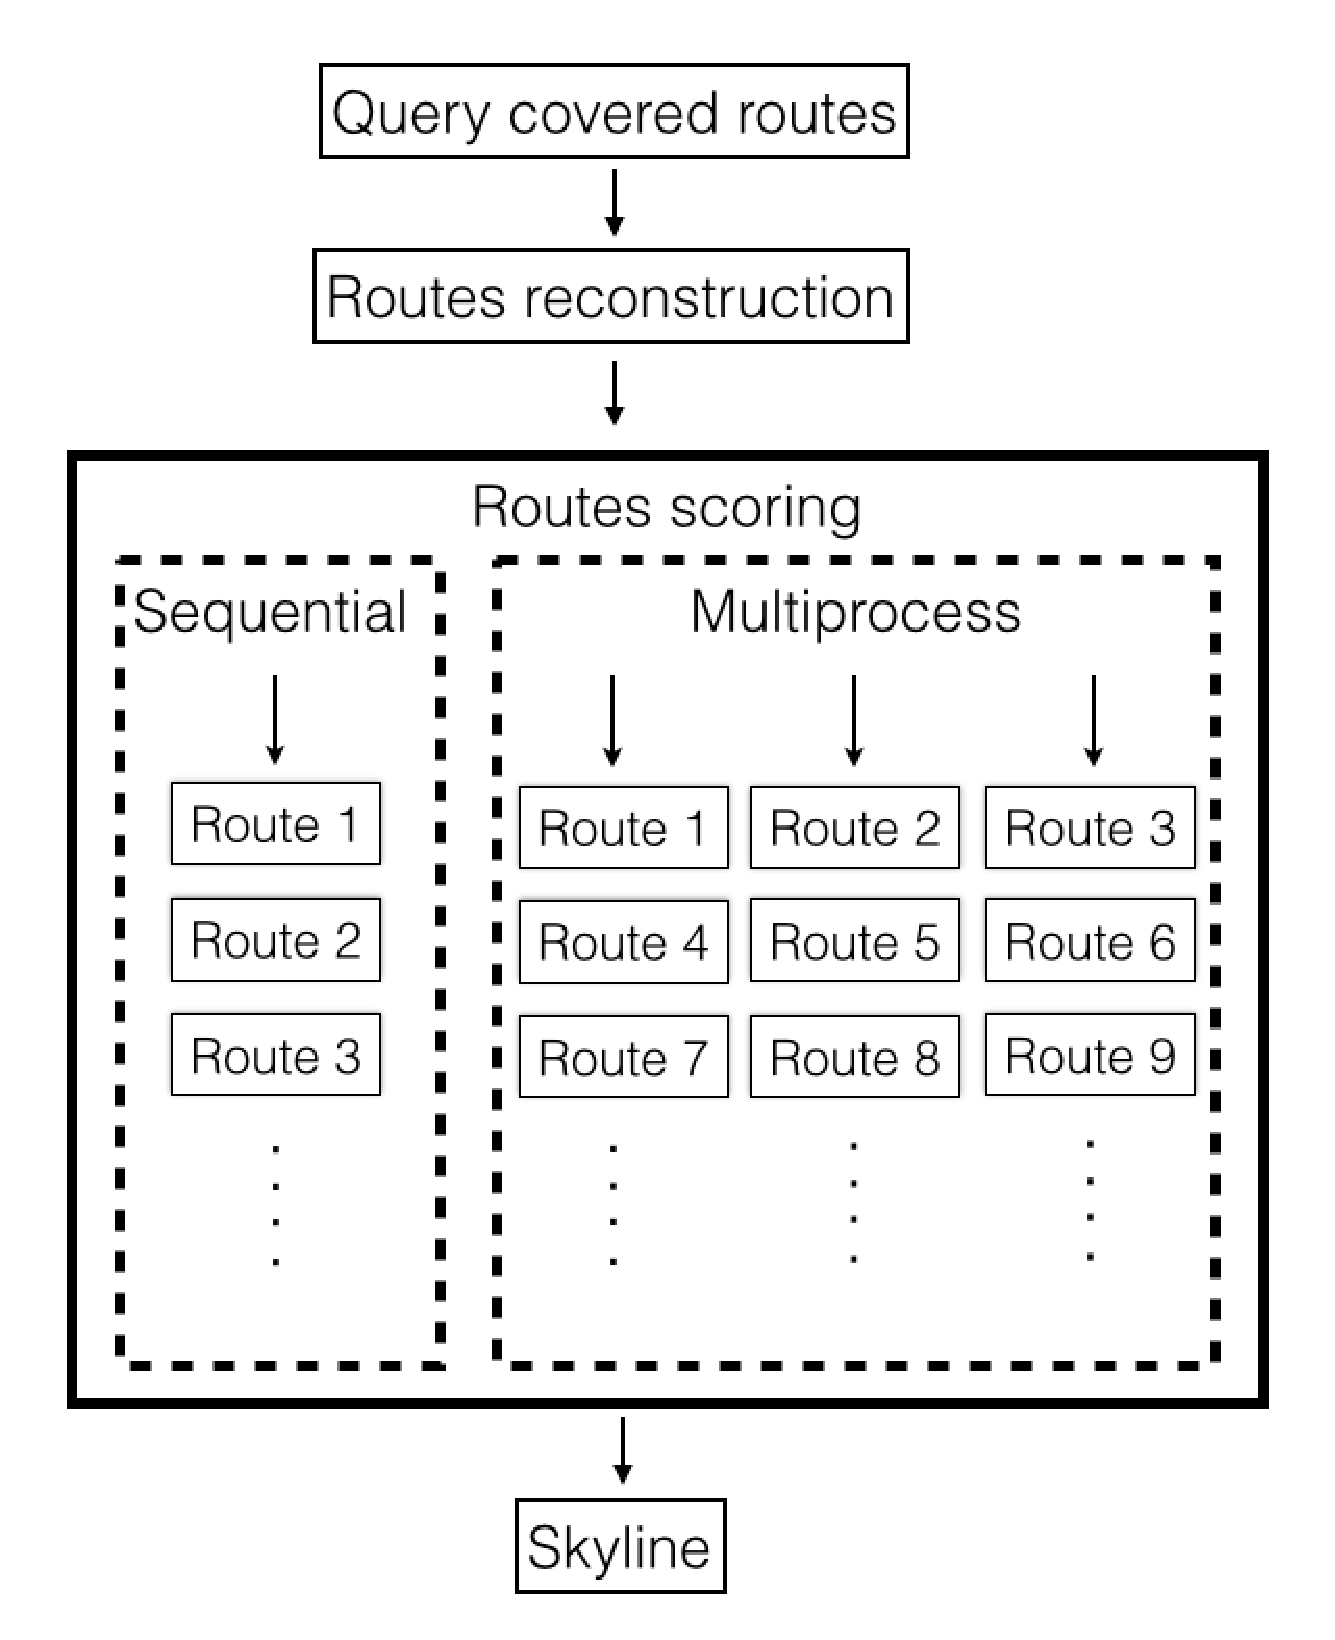
\includegraphics[width=4.5cm]{implementation.eps}
% \caption{Muiti-processing in system implementation.}
% \label{fig:implementaion}
% \end{figure}

% Data structure
